\documentclass{ximera}

\title{Gradient Descent Applet}
\author{Zack Reed}

\begin{document}
\begin{abstract}
In this activity we engage with an applet that dynamically explores the use of gradient descent to linearly fit a line to data.
\end{abstract}
\maketitle

\section*{The Main Goal: Approximating Data With a Line}

In this activity you can dynamically explore gradient descent and how it can be used to minimize the error created in some approximation process.

Here, the task is to define a line that as closely as possible runs through a set of data points. The line will be defined by two parameters: the slope $m$ and the $y$-intercept $b$. The error in the approximation is defined as the sum of the squared vertical distances from each data point to the line.

For instance, for the following 20 data points found in the graph below:

%a tikz image of data points
\begin{center}
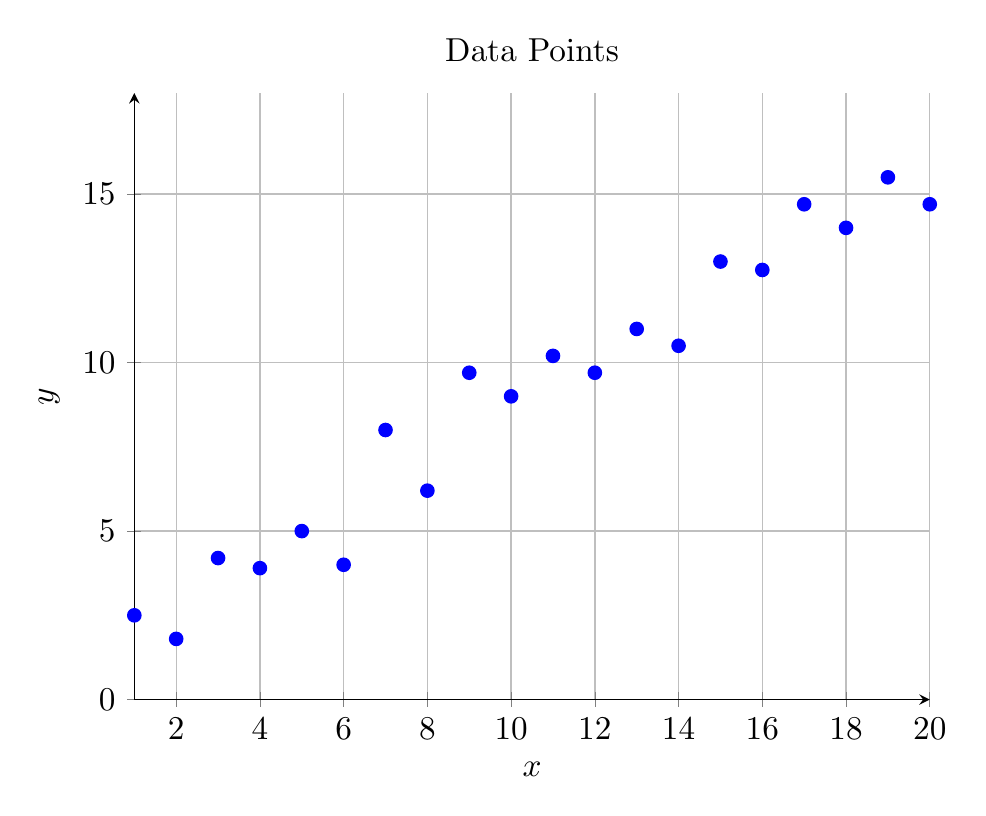
\begin{tikzpicture}[scale=1.2]
    \begin{axis}[
        axis lines = left,
        xlabel = $x$,
        ylabel = {$y$},
        title = {Data Points},
        width=10cm,
        height=8cm,
        grid=major,
        ymin=0, ymax=18,
    ]
    \addplot[only marks, mark=*, blue] coordinates {
        (1,2.5) (2,1.8) (3,4.2) (4,3.9) (5,5)
        (6,4) (7,8) (8,6.2) (9,9.7) (10,9)
        (11,10.2) (12,9.7) (13,11) (14,10.5) (15,13)
        (16,12.75) (17,14.7) (18,14) (19,15.5) (20,14.7)
    };
    \end{axis}
\end{tikzpicture}
\end{center}

we want to find the line $y = mx + b$ that minimizes the error between the height of the line and the height of each data point.

%a tikz image of data points and a line and the error lines
\begin{center}
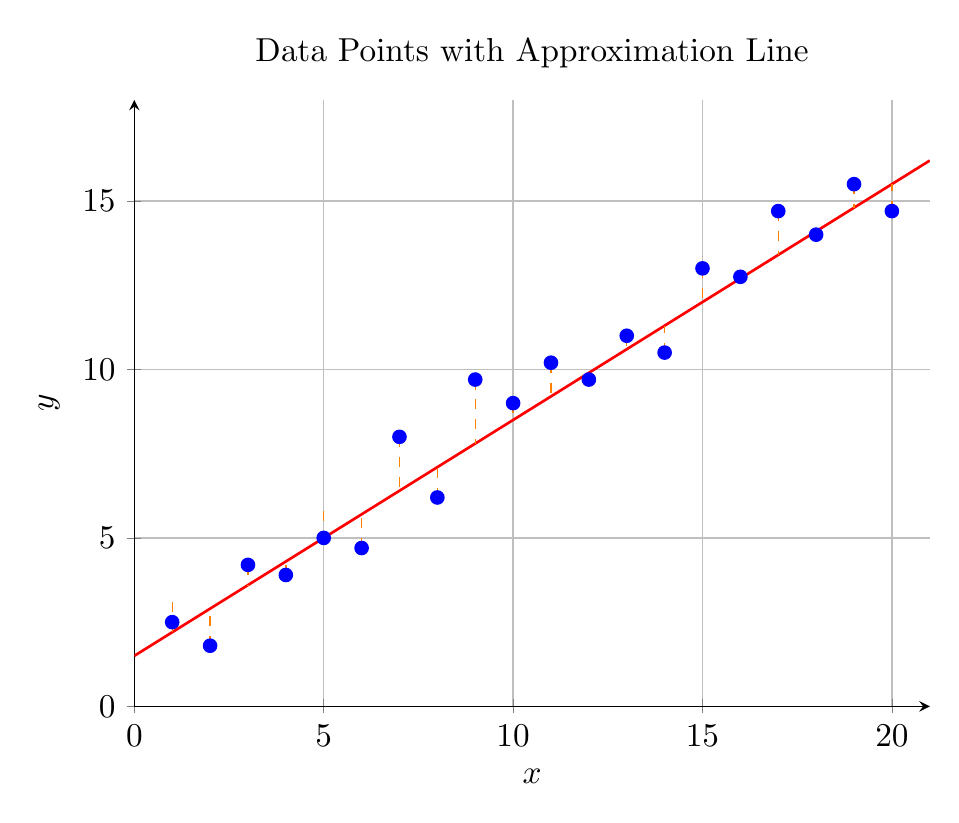
\begin{tikzpicture}[scale=1.2]
    \begin{axis}[
        axis lines = left,
        xlabel = $x$,
        ylabel = {$y$},
        title = {Data Points with Approximation Line},
        width=10cm,
        height=8cm,
        grid=major,
        ymin=0, ymax=18,
    ]
    \addplot[only marks, mark=*, blue] coordinates {
        (1,2.5) (2,1.8) (3,4.2) (4,3.9) (5,5)
        (6,4.7) (7,8) (8,6.2) (9,9.7) (10,9)
        (11,10.2) (12,9.7) (13,11) (14,10.5) (15,13)
        (16,12.75) (17,14.7) (18,14) (19,15.5) (20,14.7)
    };
    \addplot[red, thick, domain=0:21] {0.7*x + 1.5}; % Example line
    \addplot[orange, dashed] coordinates {(1,3.1) (1,2.2)};
    \addplot[orange, dashed] coordinates {(2,1.8) (2,2.9)};
    \addplot[orange, dashed] coordinates {(3,4.2) (3,3.6)};
    \addplot[orange, dashed] coordinates {(4,3.9) (4,4.3)};
    \addplot[orange, dashed] coordinates {(5,5.8) (5,5.0)};
    \addplot[orange, dashed] coordinates {(6,4.7) (6,5.7)};
    \addplot[orange, dashed] coordinates {(7,8) (7,6.4)};
    \addplot[orange, dashed] coordinates {(8,6.2) (8,7.1)};
    \addplot[orange, dashed] coordinates {(9,9.7) (9,7.8)};
    \addplot[orange, dashed] coordinates {(10,9) (10,8.5)};
    \addplot[orange, dashed] coordinates {(11,10.2) (11,9.2)};
    \addplot[orange, dashed] coordinates {(12,9.7) (12,9.9)};
    \addplot[orange, dashed] coordinates {(13,11) (13,10.6)};
    \addplot[orange, dashed] coordinates {(14,10.5) (14,11.3)};
    \addplot[orange, dashed] coordinates {(15,13) (15,12.0)};
    \addplot[orange, dashed] coordinates {(16,12.75) (16,12.7)};
    \addplot[orange, dashed] coordinates {(17,14.7) (17,13.4)};
    \addplot[orange, dashed] coordinates {(18,14) (18,14.1)};
    \addplot[orange, dashed] coordinates {(19,15.5) (19,14.8)};
    \addplot[orange, dashed] coordinates {(20,14.7) (20,15.5)};
    \end{axis}
\end{tikzpicture}
\end{center}

The orange dashed lines represent the vertical distances from each data point to the line $y = 0.7x + 1.5$. While the details of how the error is calculated are not important for this activity, it is important to note that the error is a function of the parameters $m$ and $b$ that define the line. In this case, the mean squared error (MSE) for the line $y = 0.7x + 1.5$ is approximately $.7861$.

In the language of multi-variable calculus, the function $E(m,b)$ represents the error between all possible lines of slope $m$ and intercept $b$ and the data points. For the current line $y = 0.7x + 1.5$, we have $E(0.7, 1.5) \approx 0.7861$.

Our goal is to use gradient descent to find the values of $m$ and $b$ that minimize the error function $E(m,b)$.

\section*{The Error Surface}

The error for any choice of slope $m$ and intercept $b$ creates a 3D surface, often called the "loss surface" or "error surface". For our example here, this surface has a bowl shape with a single minimum point corresponding to the best-fit line.

\begin{center}
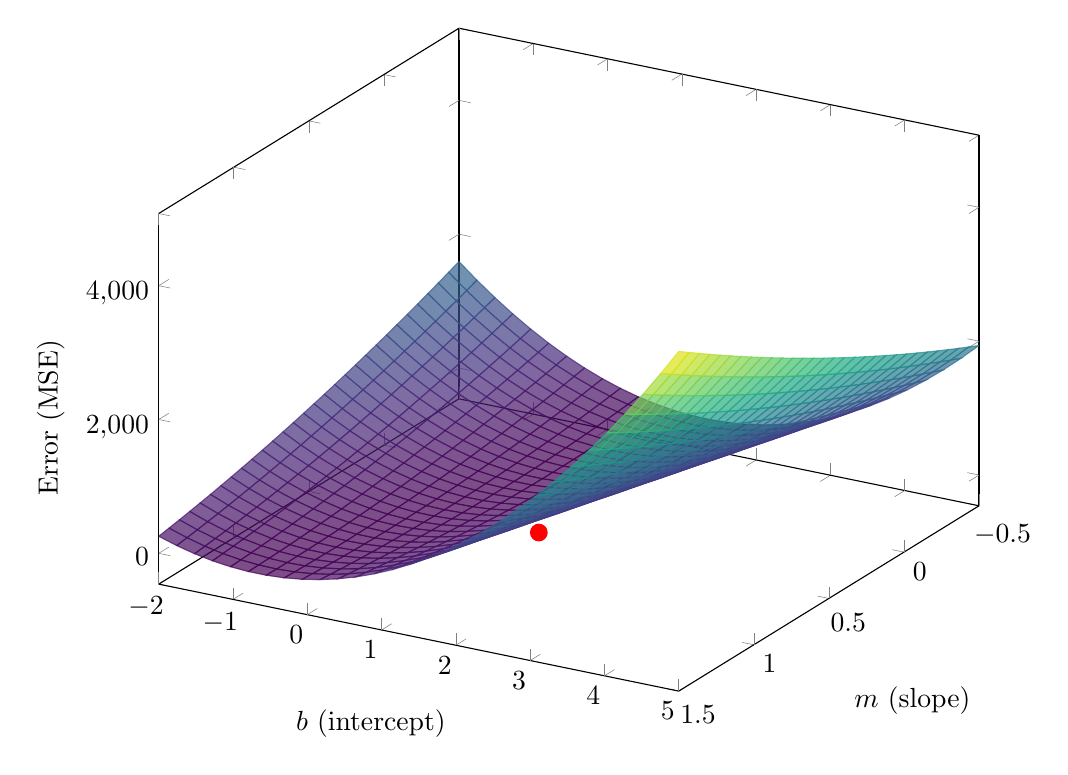
\begin{tikzpicture}
    \begin{axis}[
        view={120}{30},
        xlabel=$m$ (slope),
        ylabel=$b$ (intercept),
        zlabel={Error (MSE)},
        width=12cm,
        height=10cm,
        colormap/viridis,
    ]
    \addplot3[surf, opacity=0.7, shader=flat, domain=-0.5:1.5, domain y=-2:5, samples=30] 
        {((1*(x+y)-3.1)^2 + (2*(x+y)-1.8)^2 + (3*(x+y)-4.2)^2 + (4*(x+y)-3.9)^2 + 
            (5*(x+y)-5)^2 + (6*(x+y)-4.7)^2 + (7*(x+y)-8)^2 + (8*(x+y)-6.2)^2 + 
            (9*(x+y)-9.7)^2 + (10*(x+y)-9)^2 + (11*(x+y)-10.2)^2 + (12*(x+y)-9.7)^2 + 
            (13*(x+y)-11)^2 + (14*(x+y)-10.5)^2 + (15*(x+y)-13)^2 + (16*(x+y)-12.75)^2 + 
            (17*(x+y)-14.7)^2 + (18*(x+y)-14)^2 + (19*(x+y)-15.5)^2 + (20*(x+y)-14.7)^2)/20};
    \addplot3[only marks, mark=*, mark size=3, color=red] coordinates {(0.7, 1.5, 2.4)};
    \end{axis}
\end{tikzpicture}
\end{center}

The red point on the surface represents the error at $m=0.7$, $b=1.5$. Gradient descent is an algorithm that starts at some point on this surface and iteratively moves "downhill" (in the direction of steepest descent) to find the minimum.

\section*{Engaging with the Applet}

The following applet allows you to interactively explore how gradient descent works in this context.

For technical reasons, the applet can be found at the following link, on the author's website ``applets for learning math'':
%link to https://zackreed.github.io/applets_for_learning_math/pages/gradient-descent-walkthrough.html
\begin{center}
\href{https://zackreed.github.io/applets_for_learning_math/pages/gradient-descent-walkthrough.html}{Gradient Descent Applet}
\end{center}

There will be some interactive questions associated with the applet on the applet page, you can refer to the following video for a walkthrough of the applet and questions:

% \begin{center}
% \href{https://www.youtube.com/watch?v=example}{Gradient Descent Applet Walkthrough Video}
% \end{center}

\end{document}
